\section{Task 2: Unsupervised Domain Adaptation}

\subsection{Experimental Setup}
% Brief 2-3 sentence overview: PACS (Photo / Art Painting / Cartoon as labelled sources,
% Sketch as the unlabelled target), ResNet-18 with ImageNet initialisation and a
% seven-class head fine-tuned end to end, frozen BatchNorm running statistics, AdamW at
% lr 1e-4 / weight decay 1e-4, at most 30 epochs with patience 5 on mean source-validation
% macro-F1, domain-balanced batches of 8 per source domain plus 24 target images, seed 6304.

\begin{table}[t]
  \caption{Source-only ERM and the three adaptation methods on PACS with Sketch as the
  unlabelled target. Source columns give macro-F1 on each held-out source validation split
  (a stratified 20\% of each source domain, seed 6304) and their mean, which is the only
  quantity used for checkpoint selection. Target columns give accuracy and macro-F1 on the
  complete Sketch domain, evaluated once after every configuration and checkpoint was
  frozen, together with the change in target accuracy relative to Source-only ERM.
  Separability is the held-out accuracy of a balanced logistic-regression probe
  ($C=1$, 70/30 split, seed 6304) trained to predict source versus target from frozen
  features, so 50\% is chance and 100\% means the two domains remain perfectly
  distinguishable. Accuracy and macro-F1 diverge where a method trades performance on
  large classes for performance on small ones; macro-F1 weights all seven classes equally.}
  \label{tab:task2_methods}
  \centering
  \small
  \setlength{\tabcolsep}{5pt}
  \begin{tabular}{lcccccccc}
    \toprule
    & \multicolumn{4}{c}{\textbf{Source validation (macro-F1)}} & \multicolumn{3}{c}{\textbf{Target: Sketch}} & \\
    \cmidrule(lr){2-5} \cmidrule(lr){6-8}
    \textbf{Method} & Photo & Art & Cartoon & Mean & Acc & Macro-F1 & $\Delta$Acc & \textbf{Sep.} \\
    \midrule
    Source-only ERM         & 95.53 & 92.64 & 95.37 & 94.51 & 55.71 & 55.90 & ---      & 99.86 \\
    DAN (MMD)               & 94.88 & 88.85 & 94.56 & 92.76 & 67.80 & \textbf{66.84} & $+12.09$ & \textbf{89.70} \\
    DANN ($\alpha_{\max}=1$) & 86.73 & 80.30 & 83.25 & 83.43 & 41.51 & 36.71 & $-14.20$ & 100.00 \\
    CDAN                    & 93.87 & 90.26 & 94.12 & 92.75 & 62.36 & 63.12 & $+6.64$  & 98.49 \\
    \midrule
    \multicolumn{9}{l}{\textit{Controlled study: maximum gradient-reversal strength in DANN}} \\
    DANN ($\alpha_{\max}=0.25$) & 96.58 & 91.31 & 94.61 & 94.17 & 28.23 & 20.40 & $-27.49$ & 100.00 \\
    DANN ($\alpha_{\max}=0.5$)  & 94.42 & 87.15 & 91.10 & 90.89 & 38.92 & 32.60 & $-16.80$ & 99.86 \\
    \bottomrule
  \end{tabular}
\end{table}

\subsection{The Source-Only Domain Gap and Its Failure Modes}

\begin{figure}[t]
  \centering
  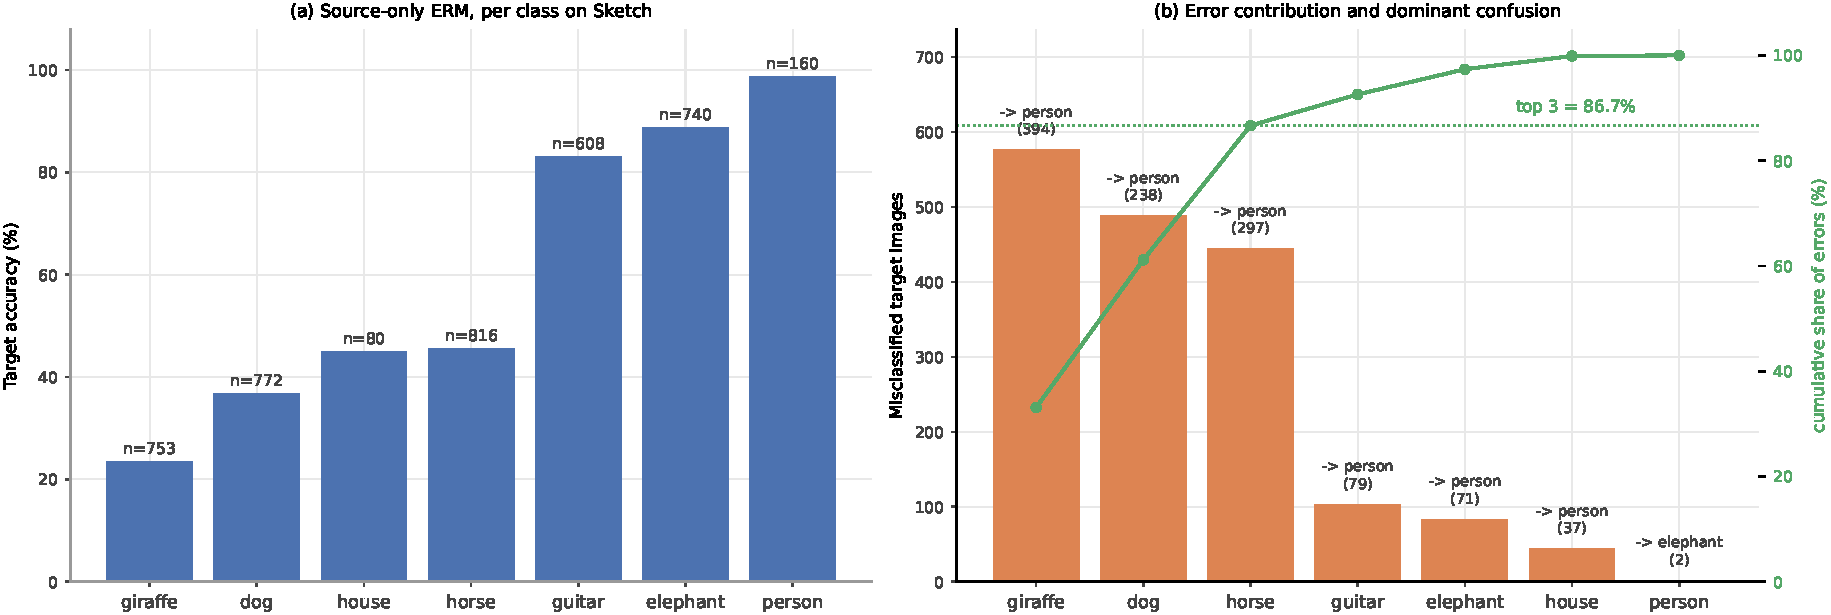
\includegraphics[width=\textwidth]{figures/task2/fig1_erm_failures.pdf}
  \caption{Where the source-only model's target errors originate.
  (a) Per-class accuracy of Source-only ERM on the Sketch domain, ordered from weakest to
  strongest, with the number of target images of each class annotated above the bar.
  Support matters for interpretation: \texttt{house} and \texttt{horse} reach almost the
  same accuracy, but \texttt{house} has only 80 target images against \texttt{horse}'s 816.
  (b) The same result expressed as misclassified images, ordered largest first, with the
  cumulative share of all target errors overlaid (right axis). The dotted line marks the
  contribution of the three largest error sources. Each bar is annotated with the class
  that absorbs most of those errors and the number of such predictions, which shows that
  six of the seven classes send their dominant confusion to \texttt{person}.}
  \label{fig:task2_erm_failures}
\end{figure}

The source-only ERM showed a substantial domain gap of 38.61 points (macro-F1) between the source and target domains. Although the model achieved a good 94.51\% macro-F1 on the source domain, on the target (Sketch domain), it only attained 55.90\%. The model showed a healthy decrease in training loss from 0.477 to 0.049, respectively observed an increase in training accuracy up to 98.79\%, and a reflective increase in source-validation macro-F1, peaking at 94.51\% at epoch 11. The performance remained consistently high across the source domains (Photo at 95.53\%, Art Painting at 92.64\%, and Cartoon at 95.37\%). This demonstrates that ERM made the model learn class-discriminative source-domain features; however, these features are not directly transferable to the target domain and contain strong domain-specific information, which is clearly visible in the 99.86\% domain-separability score.

The classes that resulted in the most important target failures were found by accounting for the overall error share of each class. As per these numbers, Giraffe, Dog, and Horse accounted for 86.7\% of the overall errors on the target domain. Additionally, the model also displayed a strong bias towards the person class, and the model confused the majority of the classes with person, producing around 1,116 such errors. In contrast, the elephant and guitar classes showed good results, obtaining 88.78\% and 83.06\% accuracy. This shows that the domain shift did not affect each class uniformly.

\subsection{Domain Separability and Target Recognition}

\begin{figure}[t]
  \centering
  \begin{minipage}[t]{0.46\textwidth}
    \centering
    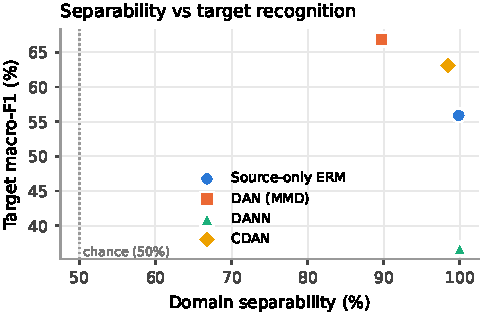
\includegraphics[width=\textwidth]{figures/task2/fig3_separability.pdf}
  \end{minipage}\hfill
  \begin{minipage}[t]{0.52\textwidth}
    \centering
    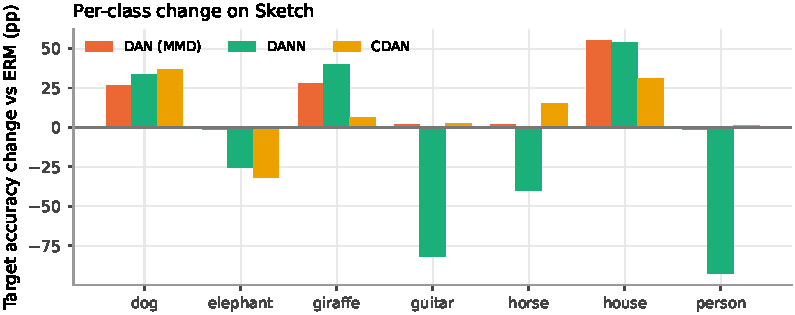
\includegraphics[width=\textwidth]{figures/task2/fig4_per_class.pdf}
  \end{minipage}
  \caption{Aggregate and class-level evidence on whether reduced domain separability
  corresponds to improved target recognition. \textbf{Left:} target macro-F1 against domain
  separability for the four methods; the dotted line marks chance separability (50\%).
  Only DAN moves appreciably away from the 100\% ceiling, and it also achieves the highest
  target macro-F1, but CDAN improves on Source-only ERM while remaining at 98.49\%
  separability, so reduced separability is not a precondition for successful adaptation.
  \textbf{Right:} change in per-class target accuracy relative to Source-only ERM, in
  percentage points, for each adaptation method. Bars above zero indicate positive transfer
  and bars below zero negative transfer. DAN and CDAN improve five and six of the seven
  classes respectively, while DANN's aggregate collapse is concentrated in
  \texttt{guitar}, \texttt{person} and \texttt{horse}.}
  \label{fig:task2_separability}
\end{figure}

After the linear probe via logistic regression, we got the scores reported in Table~\ref{tab:task2_methods}. Across all methods, we see a clear enough pattern: the higher the domain separability between source and target domains, the lower the target accuracy scores. ERM set the baseline for separability at around 99.86, with the target accuracy at 55.71 points. The treatment methods like DAN and CDAN were able to fractionally reduce this separability gap, and as the domain separability scores reduced with these methods, so did the accuracy on the target domain improve. DANN, though it performed miserably because of an unstable optimization flow, shows that it has the highest domain separability score and thus has the lowest target-domain accuracy.

The effect of domain separability is clearly visible in the class-level results as well. The methods that performed better compared to the others, like DAN or CDAN, showed successful adaptation. However, this improvement was not uniform across all of the classes. In DAN, the adaptation improved 5 out of 7 classes, with giraffe improving by 27.89 points, house by 55.00 points, and dog by 26.81 points. However, for elephants and persons, it exhibited negative transfer, declining in performance by 1.62 and 1.25 points. Similarly, CDAN also adapted successfully overall and improved 6 out of 7 classes, except elephant, where its performance decreased by 31.62 points. DANN displayed negative transfer overall. Despite showing adaptation on dog, giraffe, and house, it reported terrible performance on guitar, person, horse, and elephant. Its target macro-F1 plummeted by 19.19 points relative to ERM, most likely because of the instability it faced during optimization.

Overall, reduced domain separability can be associated with better performance on target recognition for DAN and CDAN. However, for good adaptation, per-class performance matters as well.

\subsection{Class-Conditional versus Marginal Alignment}

The results do not clearly support the claim that class conditioning helps preserve class semantic features better. The treatment methods DAN and DANN use two different approaches for domain alignment, where DAN uses MMD to compare distance between the source and target distributions and uses it as a loss penalty, i.e., the larger the distance between the source and target domain distributions, the greater the loss penalty, forcing the model to learn features that bring the two distributions closer in vector space so that the feature extractor learns about features that have resulted in a reduced gap between the distributions. With DAN, the domain separability score reduced down to 89.69 from 99.86 and showed the best target adaptation performance, reaching 66.84\% macro-F1; however, the individual class-wise macro-F1 for DAN is not uniform across the classes, as it performed really well on 5 out of 7 classes (with giraffe $+27.89$, house $+55.00$, and dog $+26.81$ points), and for elephant and person, it saw a marginal decline. CDAN also observed an improved domain adaptation and reached a 63.12\% target macro-F1, marginally less than DAN. Overall, it performed well on 6 out of 7 classes and also preserved person and guitar recognition, improving them by 1.25 and 2.47 points, but reduced the adaptation on the elephant class by a massive 31.62 points, and also provided just a 6.51-point gain on the giraffe, whereas on the same giraffe class DAN improved the adaptation by 27.89 points. Thus, the class conditionality might have partially preserved the class-wise consistency, with 6 classes improving; however, it did not manage to improve the overall aggregate for target adaptation.

CDAN does outperform the marginal adversarial alignment DANN, where DANN only reported 36.71\% macro-F1. DANN also diverged with extremely larger classification and alignment losses and the optimizational instability, which is a key confounding factor in the underperforming DANN. Overall results may suggest that conditioning can better preserve semantic structure, and it improved aggregate target adaptation relative to ERM but did not outperform DAN, and stable DAN depicted a good marginal alignment that may outperform CDAN.

\subsection{Effect of Increasing Alignment Strength}

\begin{figure}[t]
  \centering
  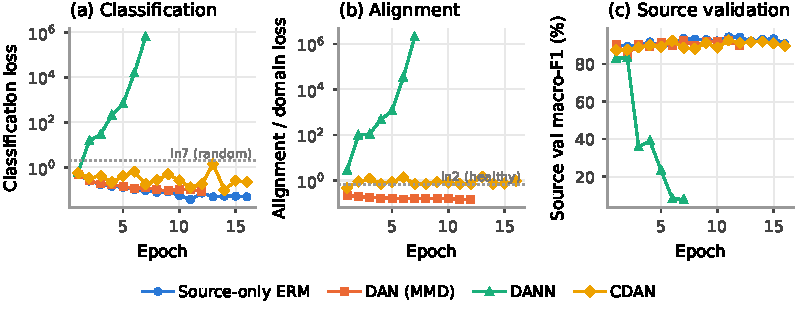
\includegraphics[width=\textwidth]{figures/task2/fig2_training_curves.pdf}
  \caption{Training behaviour of the four methods, on logarithmic axes for the two losses.
  (a) Classification loss on the labelled source batches. The dotted line marks
  $\ln 7 = 1.946$, the value a seven-class classifier attains by predicting uniformly, so
  a curve above it is assigning less probability to the correct class than random guessing
  would. (b) Alignment loss: the MMD penalty for DAN and the domain-classification loss for
  DANN and CDAN. The dotted line marks $\ln 2 = 0.693$, the value a domain discriminator
  attains when it genuinely cannot distinguish the two domains, which is the equilibrium
  adversarial alignment aims for. CDAN remains close to this value throughout, whereas
  DANN departs from it from the second epoch onward. (c) Mean source-validation macro-F1,
  the quantity used for checkpoint selection. DANN's losses diverge during epoch~2 while
  its source validation is still at its maximum, so the collapse is visible internally one
  epoch before the selection signal reflects it.}
  \label{fig:task2_training}
\end{figure}

\begin{figure}[t]
  \centering
  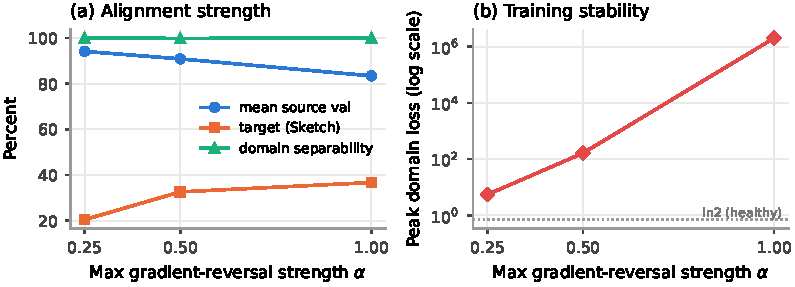
\includegraphics[width=0.72\textwidth]{figures/task2/fig5_alignment_study.pdf}
  \caption{Controlled study over the maximum gradient-reversal strength
  $\alpha_{\max}\in\{0.25,0.5,1\}$ in DANN, with every other setting held fixed. Source
  macro-F1, target macro-F1 and domain separability are shown on a common percentage axis,
  with the Source-only ERM target macro-F1 marked for reference. Increasing alignment
  strength raises target macro-F1 and lowers source macro-F1, while separability stays at
  approximately 100\% at all three settings, so the mechanism the objective is intended to
  produce is not observed at any strength. All three settings remain below the Source-only
  baseline on the target.}
  \label{fig:task2_alignment_study}
\end{figure}

Overall baseline model performance with DANN, having alignment strength = 1.0, started well in the very first epoch. At the end of epoch 1, the classification loss was 0.61 (well below $\ln(7)=1.946$), training accuracy reached 80.95\%, and validation F1 reached 83.21\%. Meanwhile, the alignment loss reached 2.78 (exceeding $\ln(2)=0.693$), while domain accuracy settled at 58.18\%. However, from epoch 2 onwards, the overall optimization became unstable, as the model's classification loss shot up to 15.21 in the second epoch; the training accuracy dropped to 69.80\%, while the validation F1 moved up to 83.43\%, which tells us the model is making some very confident errors as its training accuracy decreases while its validation score remains high. Source-validation performance then collapsed outright from the 3rd epoch, when the validation macro-F1 plummeted from 83.43\% down to 35.96\% and then eventually reached 7.83\%. Both the probabilistic loss and classification performance now show a total failure. The domain accuracy stayed between 42.29\% and 58.18\%; however, the alignment loss increased from 2.78 at the end of the first epoch to 97.49 in the second, reaching 2,013,773.19 in 7 epochs.

As we halve DANN's alignment strength, things do start to get a little better for the source-domain accuracy, as the source macro-F1 gained 7.46 points; however, the reduced alignment strength impacted the target macro-F1, decreasing it by 4.11 points. The pattern repeats when we further reduce the alignment strength, which further increases the model accuracy on source classification; however, it progressively damages target recognition, decreasing target macro-F1 by another 12.19 points. Interestingly, while we have these variations in target F1 score as we decrease the alignment strength, source and target separability remains around 100\%. Therefore, in this scenario, the stronger or weaker adversarial objective failed to produce any measurable domain-invariant features.

In fact, all three DANN configurations remained well below the ERM target macro-F1 of 55.90\%. So, the trade-off between low and high alignment strength had a substantial positive effect on target macro-F1 within the DANN variants; however, stronger alignment destabilized the model's training, and a smaller value further deteriorated the target macro-F1.
